\begin{frame}
    \frametitle{題幹}

    課本翻譯太爛,見 \texttt{7\_15 重新翻譯.pdf}
    
\end{frame}

\begin{frame}
    \frametitle{斷點回歸 Regression Discontinuity}
    \begin{columns}
        \begin{column}{0.6\textwidth}
            \begin{figure}
                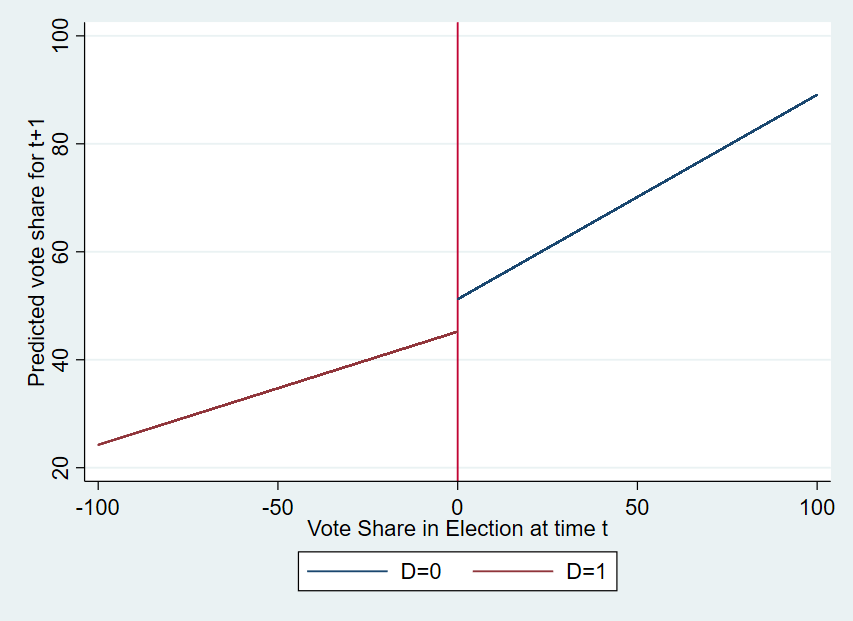
\includegraphics[width=\textwidth]{../Results/7_15_b.png}
            \end{figure}        
        \end{column}

        \begin{column}{0.4\textwidth}
            \begin{align*}
                Y &= \alpha_1 + \alpha_2 X + D(\beta_1 + \beta_2 X) \\
                &=reg~Y ~X~D~XD
            \end{align*}
        \end{column}
    \end{columns}
    


    

\end{frame}